\begin{figure}[t!]
    \centering
    \begin{subfigure}[b]{\linewidth}
        \centering
        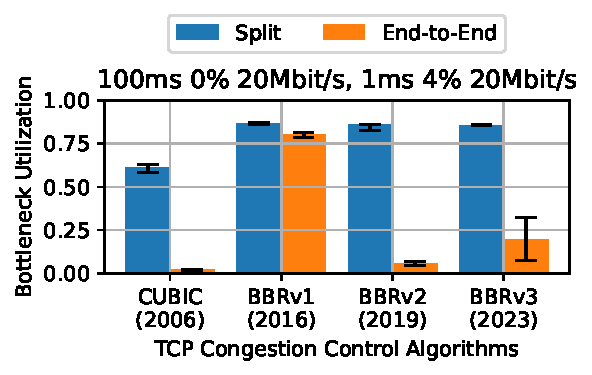
\includegraphics[width=0.5\linewidth]
         {splitting/figures/bbr_over_time_network_20_20_100_1_None_None_0_4.pdf}
        \captionsetup{skip=0pt}
        \caption{Asymmetric, lossy last-mile.}
        \label{fig:splitting:bbr-over-time:class1}
    \end{subfigure}
    \begin{subfigure}[b]{\linewidth}
        \centering
        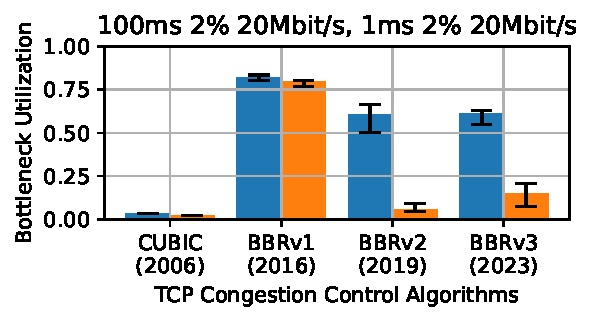
\includegraphics[width=0.5\linewidth]
         {splitting/figures/bbr_over_time_network_20_20_100_1_None_None_2_2.pdf}
        \captionsetup{skip=0pt}
        \caption{Asymmetric, both path segments are lossy.}
        \label{fig:splitting:bbr-over-time:class2}
    \end{subfigure}
    \begin{subfigure}[b]{\linewidth}
        \centering
        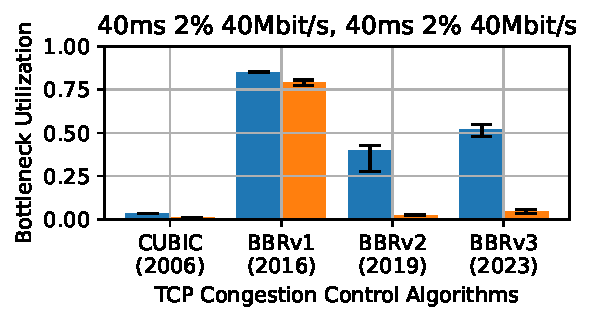
\includegraphics[width=0.5\linewidth]
         {splitting/figures/bbr_over_time_network_40_40_40_40_None_None_2_2.pdf}
        \captionsetup{skip=0pt}
        \caption{Symmetric, both path segments are lossy.}
        \label{fig:splitting:bbr-over-time:class3}
    \end{subfigure}
    \caption{Three classes of network settings in which the throughput of a
     long-lived data transfer using BBRv3 benefits significantly from
     connection-splitting. While the throughput of TCP using BBRv1 may not have
     benefitted from a PEP, as the BBR algorithm has evolved over time, it has
     also made connection-splitting pertinent again. In two of these classes,
     split BBRv3 even achieves high bottleneck link rate utilization where split
     CUBIC does not. IQR of $n=20$.}
    \label{fig:splitting:bbr-over-time}
\end{figure}
